        \documentclass{standalone}
        \usepackage{../BlogTikz}
        \begin{document}

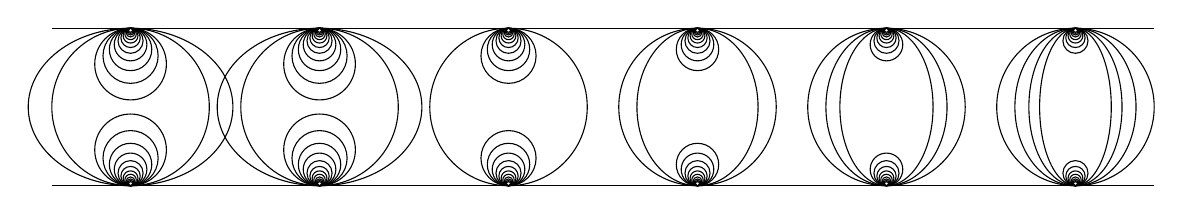
\begin{tikzpicture}
	\tikzset{
		pics/hawaiian/.style args={#1,#2,#3,#4,#5,#6}{
			code={
				\ifthenelse{\equal{#4}{0}}{}{
					\foreach \x in {1,...,#4}
					\draw (#1,#2) ellipse ({#3*(1/1.3^(\x-1))} and #3);
				}
				\foreach \x in {#5,...,#6}{
					\draw (#1,#2-#3+#3/1.3^\x) circle (#3/1.3^\x);
					\draw (#1,#2+#3-#3/1.3^\x) circle (#3/1.3^\x);
				}
	}}}
	\draw (-7,-1)--(7,-1) (-7,1)--(7,1);
	\pic {hawaiian={-6,0,1,0,3,14}};
	\pic {hawaiian={-3.6,0,1,0,3,14}};
	\pic {hawaiian={-1.2,0,1,1,4,14}};
	\pic {hawaiian={1.2,0,1,2,5,14}};
	\pic {hawaiian={3.6,0,1,3,6,14}};
	\pic {hawaiian={6,0,1,4,7,14}};
\end{tikzpicture}
        \end{document}
